\documentclass{standalone}
\usepackage{tikz}
\usetikzlibrary{trees}
\begin{document}
\tikzstyle{every node}=[anchor=west, text width=12ex]
 \small
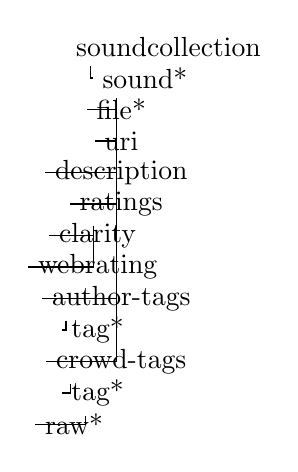
\begin{tikzpicture}[%
  grow via three points={one child at (-0.3,-0.4) and
  two children at (-0.3,-0.4) and (-0.3,-0.8)},
  edge from parent path={([xshift=2ex] \tikzparentnode.south west) |- (\tikzchildnode.west)}]
 
  \node {soundcollection}
    child { node {sound*}
    	child { node {file*}}
	child { node {uri}}
	child { node {description}}
	child { node {ratings}
	   child { node {clarity}}
	   child { node {webrating}}
	   }
	child [missing] {}
	child [missing] {}
	child { node {author-tags}
	   child { node {tag*}}
	   }
	child [missing] {}
	child { node {crowd-tags}
	   child { node {tag*}
	      child { node {raw*}}
	      }
	   }
	};
\end{tikzpicture}
\end{document}